Implementemos el siguiente sistema en MATLAB y Simulink:

\begin{equation}
    G(s) = \frac{e^{-5s}}{s + 2}
\end{equation}

\begin{figure}[htbp]
    \centering
    \captionsetup{font=small}
    \captionsetup[subfigure]{justification=centering}

    \makebox[0.48\linewidth]{\large\bfseries MATLAB}%
    \hfill
    \makebox[0.48\linewidth]{\large\bfseries Simulink}

    \par\medskip

    \begin{minipage}[c]{0.48\linewidth}
\begin{lstlisting}
clc;
clear all;
close all;

% Funcion de transferencia
s = tf('s');
G = exp(-5*s)/(s + 2);

[yg, tg] = step(G);
\end{lstlisting}
    \end{minipage}%
    \hfill
    \begin{minipage}[c]{0.48\linewidth}
        \centering

        \includegraphics[
            width=0.95\linewidth,
            height=3.5cm,
            keepaspectratio
        ]{imagenes/sistema.png}
    \end{minipage}

    \par\bigskip


    \begin{subfigure}[t]{0.48\linewidth}
        \vspace{0pt}
        \centering

        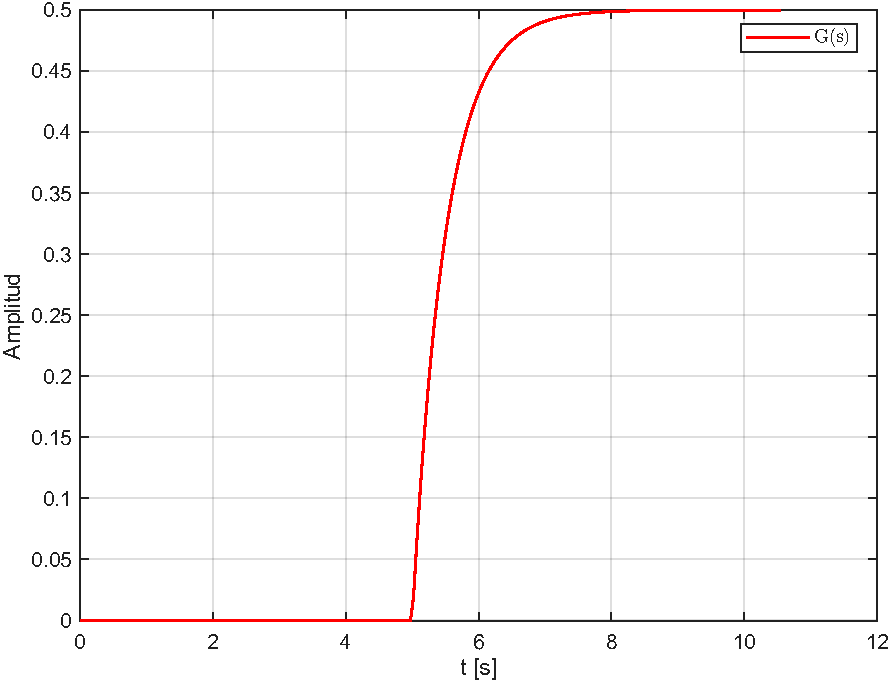
\includegraphics[width=\linewidth]
            {imagenes/ploteo_con_matlab.pdf}

        \caption{Respuesta obtenida con MATLAB.}
        \label{fig:respuesta-matlab}
    \end{subfigure}%
    \hfill
    \begin{subfigure}[t]{0.48\linewidth}
        \vspace{0pt}
        \centering

        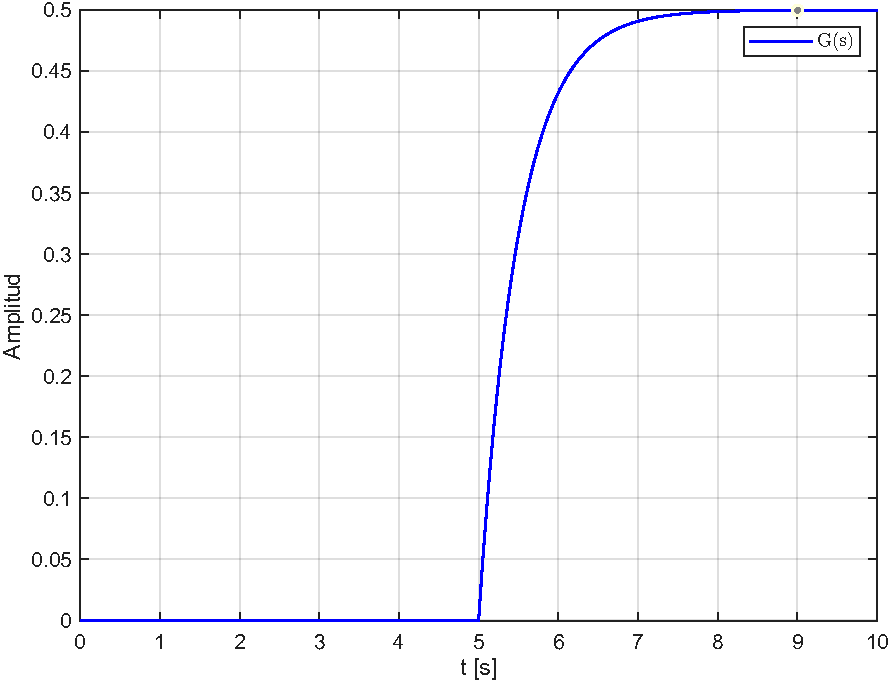
\includegraphics[width=\linewidth]
            {imagenes/ploteo_con_simulink.pdf}

        \caption{Respuesta obtenida con Simulink.}
        \label{fig:respuesta-simulink}
    \end{subfigure}

    \caption{Comparación de la respuesta al escalón del sistema
    $G(s)=e^{-5s}/(s+2)$ mediante MATLAB y Simulink. Las respuestas son iguales}
    \label{fig:comparacion-matlab-simulink}
\end{figure}



El siguiente código muestra cómo trabajar con funciones desde el \textit{Workspace} de MATLAB para implementar en Simulink.

\begin{lstlisting}
%Sistema desde el Workspace
t_array = 0:0.1:20;
x1 = t_array.*sin(sin(t_array)) + t_array;
x2 = t_array.^2.*exp(-0.5*t_array);

simin = [t_array', x1', x2'];
\end{lstlisting}


\texttt{simin} es una matriz de dimensión 201x3, que con el bloque \textit{From Workspace} podemos cargarlo al Simulink. Además, podemos definir otro bloque, \textit{Fcn}, que nos permite trabajar con las funciones ingresadas en el Workspace. El sistema es:


\begin{figure}[htbp]
    \centering

    \resizebox{0.5\linewidth}{!}{%
        \begin{tikzpicture}[
            font=\sffamily,
            bloque/.style={
                draw=black,
                fill=white,
                line width=0.6pt
            },
            conexion/.style={
                draw=black!45,
                line width=0.6pt,
                -{Triangle[
                    length=2.2mm,
                    width=2mm,
                    color=black
                ]}
            },
            etiqueta/.style={
                font=\sffamily\small,
                align=center
            }
        ]

            % Bloque From Workspace.
            \node[
                bloque,
                minimum width=1.8cm,
                minimum height=0.7cm
            ] (entrada) {\large simin};

            % Bloque Fcn.
            \node[
                bloque,
                minimum width=3.9cm,
                minimum height=1.1cm,
                right=2.1cm of entrada
            ] (funcion) {$\displaystyle \sin(u(1))-u(2)+10$};

            % Bloque Scope.
            \node[
                bloque,
                minimum width=0.85cm,
                minimum height=0.9cm,
                right=2.1cm of funcion
            ] (scope) {};

            % Pantalla dentro del Scope.
            \draw[
                line width=0.5pt,
                rounded corners=1.5pt
            ]
                ([xshift=1.2mm,yshift=-1.2mm]scope.north west)
                rectangle
                ([xshift=-1.2mm,yshift=-5mm]scope.north east);

            % Flechas entre los bloques.
            \draw[conexion]
                (entrada.east) -- (funcion.west);

            \draw[conexion]
                (funcion.east) -- (scope.west);

            % Etiquetas inferiores.
            \node[etiqueta, below=1.5mm of entrada]
                {From\\Workspace};

            \node[etiqueta, below=1.5mm of funcion]
                {Fcn};

            \node[etiqueta, below=1.5mm of scope]
                {Scope};

        \end{tikzpicture}%
    }
\end{figure}

Y su respuesta 

\begin{figure}[ht!]
    \centering
    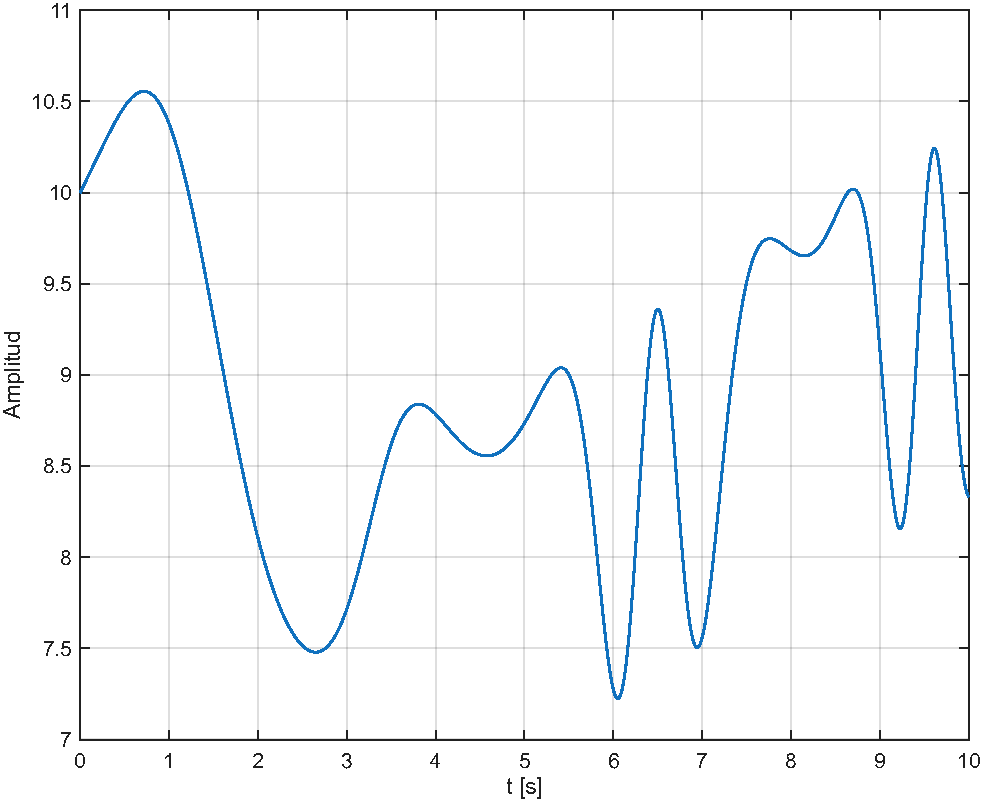
\includegraphics[width=0.8\textwidth]{imagenes/respuesta_fromworkspace.pdf}
    \caption{Salida de $\sin(u_1) - u_2 + 10$}
    \label{fig:8}
\end{figure}


Las ventajas de representar funciones de transferencias desde el Workspace es que son fáciles de manipular y definir, permitiendo una comunicación más simple entre MATLAB y Simulink. 

Por último, definamos las siguientes funciones de transferencias:

\begin{equation}
    G_1(s) = e^{-2s}\frac{3s}{s^2 + s + 2} \quad G_2(s) = \frac{1}{(s+2)(s+4)(s+5)} \quad G_3(s) = 
    \begin{cases}
        \dot{x} = Ax +Bu \\
        y = Cx + Du
    \end{cases}
\end{equation}


\noindent donde

\begin{align*}
    A &= 
    \begin{bmatrix}
        -8 & -2.5 \\
        2 & 0
    \end{bmatrix}
    \quad
    B = 
    \begin{bmatrix}
        2 \\
        0
    \end{bmatrix}
    \\[0.2cm]
    C &= [0.5 \ 0.75] \quad D = 0
\end{align*}

Implementemos el siguiente sistema y veamos su respuesta (también su código a implementar).

\begin{figure}[htbp]
    \centering

    \resizebox{\linewidth}{!}{%
        \begin{tikzpicture}[
            font=\sffamily,
            bloque/.style={
                draw=black,
                fill=white,
                line width=0.6pt,
                minimum width=2.4cm,
                minimum height=0.9cm,
                inner sep=0pt,
                drop shadow={
                    shadow xshift=0.8pt,
                    shadow yshift=-0.8pt,
                    opacity=0.25
                }
            },
            sumador/.style={
                bloque,
                circle,
                minimum size=5mm
            },
            conexion/.style={
                line width=0.45pt,
                -{Triangle[length=1.9mm,width=1.8mm]}
            },
            signo/.style={
                font=\scriptsize,
                inner sep=0pt
            }
        ]

            %-----------------------------------------
            % Bloques principales.
            %-----------------------------------------
            \node[
                bloque,
                minimum width=0.75cm,
                minimum height=0.75cm
            ] (escalon) at (0,0) {};

            \node[sumador] (suma1) at (1.65,0) {};

            \node[bloque] (G1) at (4.35,0)  {G1};
            \node[bloque] (G2) at (4.95,-2) {G2};
            \node[bloque] (G3) at (9.45,-2) {G3};

            \node[sumador] (suma2) at (11.65,0) {};

            % Scope.
            \node[
                bloque,
                minimum width=0.75cm,
                minimum height=0.8cm
            ] (scope) at (14.4,0) {};

            % Puerto de salida.
            \node[
                bloque,
                rounded corners=5pt,
                minimum width=0.75cm,
                minimum height=0.36cm
            ] (salida) at (14.4,-2) {1};

            %-----------------------------------------
            % Detalles de los bloques.
            %-----------------------------------------

            % Icono de la entrada escalon.
            \draw[black!70, line width=0.5pt]
                (-0.29,-0.24) -- (0,-0.24)
                -- (0,0.24) -- (0.29,0.24);

            % Pantalla del Scope.
            \draw[line width=0.5pt, rounded corners=1pt]
                ([xshift=1mm,yshift=-1mm]scope.north west)
                rectangle
                ([xshift=-1mm,yshift=-4.5mm]scope.north east);

            % Etiqueta debajo de G1.
            \node[anchor=north, font=\sffamily\small]
                at ([yshift=-1mm]G1.south) {LTI System};

            % Pequenos iconos grises de los bloques LTI.
            \foreach \nombre in {G1,G2,G3}{
                \begin{scope}[shift={
                    ([xshift=1.6mm,yshift=1.6mm]\nombre.south west)
                }]
                    \draw[
                        draw=black!25,
                        fill=black!12,
                        line width=0.35pt
                    ]
                        (-0.4mm,0.6mm) -- (0.4mm,0.6mm)
                        -- (0.4mm,-0.2mm) -- (1mm,-0.2mm)
                        -- (0,-1.2mm) -- (-1mm,-0.2mm)
                        -- (-0.4mm,-0.2mm) -- cycle;
                \end{scope}
            }

            %-----------------------------------------
            % Signos de los sumadores.
            %-----------------------------------------
            \node[signo]
                at ([xshift=-1.3mm]suma1.center) {$+$};

            \node[signo]
                at ([yshift=-1.3mm]suma1.center) {$-$};

            \node[signo]
                at ([xshift=-1.3mm]suma2.center) {$+$};

            \node[signo]
                at ([yshift=-1.3mm]suma2.center) {$+$};

            %-----------------------------------------
            % Puntos de derivacion.
            %-----------------------------------------
            \coordinate (toma)       at (7.25,0);
            \coordinate (reparto)    at (7.25,-2);
            \coordinate (tomasalida) at (13.1,0);

            %-----------------------------------------
            % Camino principal.
            %-----------------------------------------
            \draw[conexion] (escalon.east) -- (suma1.west);
            \draw[conexion] (suma1.east) -- (G1.west);
            \draw[conexion] (G1.east) -- (suma2.west);
            \draw[conexion] (suma2.east) -- (scope.west);

            %-----------------------------------------
            % Ramas inferiores.
            %-----------------------------------------

            % La salida de G1 alimenta a G2 y G3.
            \draw[line width=0.45pt] (toma) -- (reparto);

            \draw[conexion] (reparto) -- (G2.east);
            \draw[conexion] (reparto) -- (G3.west);

            % Realimentacion negativa mediante G2.
            \draw[conexion] (G2.west) -| (suma1.south);

            % G3 entra al segundo sumador con signo positivo.
            \draw[conexion] (G3.east) -| (suma2.south);

            % Derivacion al puerto de salida 1.
            \draw[conexion] (tomasalida) |- (salida.west);

            % Puntos negros en las uniones.
            \foreach \punto in {toma,reparto,tomasalida}{
                \fill (\punto) circle[radius=1.15pt];
            }

        \end{tikzpicture}%
    }

    \caption{Diagrama de bloques con realimentación negativa
    mediante $G_2$.}
    \label{fig:realimentacion-g1-g2-g3}
\end{figure}

\newpage

\begin{figure}[ht!]
    \centering
    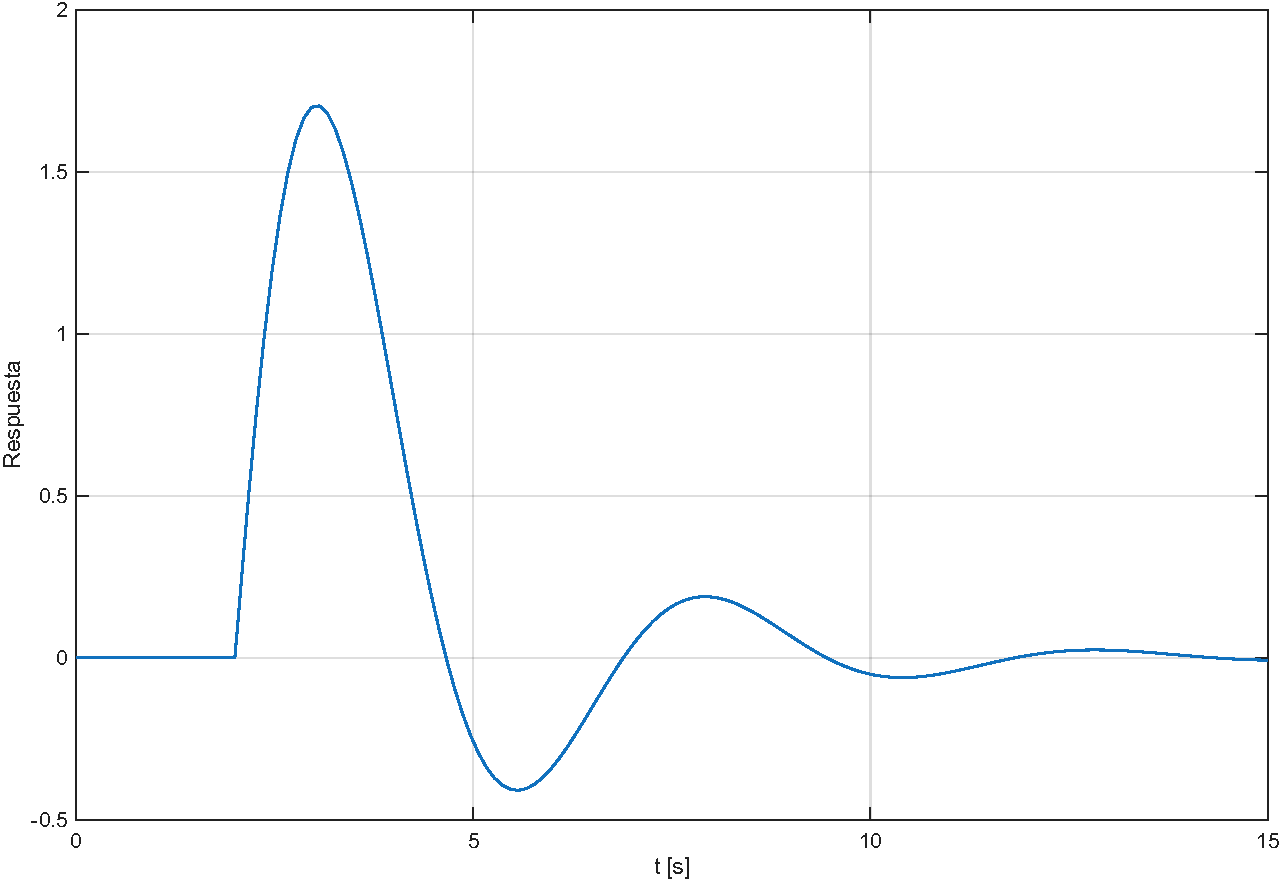
\includegraphics[width=0.8\textwidth]{imagenes/respuesta_sistema18.pdf}
    \caption{Respuesta al sistema de la figura de arriba}
    \label{fig:}
\end{figure}

\begin{lstlisting}
clc
clear all
close all

s = tf('s');
G1 = exp(-2*s)*3*s/(s^2 + s + 2);
G2 = zpk([], [-2, -4, -5], 1);

A = [-8, -2.5;
      2,    0];

B = [2;
     0];

C = [0.5, 0.75];
D = [0];

G3 = ss(A, B, C, D); 

%salida
sis = sim('mod_18.slx');

%%
data = sis.yout.extractTimetable;
plot(sis.tout, data.Data)
\end{lstlisting}
